\section{Persona}
\label{sec:persona}

As result of our needfinding, we came up with a unified persona encapsulating our insights and identified needs that we focus on in the following chapters. A picture of our persona can be found in figure \ref{fig:persona}.

%{Jonathan} Not nesseary here yet and confusing
%In 3-5 years, 
Linda Becker is 35 years old. She is a senior developer, married and has a 10 year old daughter. They own an Audi A3 sedan and a Q7 SUV which they both share depending on what they need the car for. This also means that they sometimes have communication problems about the state of the different cars if Linda takes a car that her husband had taken before her. For example she sometimes wonders about the gas level if she cannot immediately ask her husband about it. This is important for her so she can plan to gas up the car. Other examples for such problems are icy windows or important maintenance that need to be planned into the schedule as well. Her husband is more often worried about the safety of the car, for example whether it was locked correctly. He would like to have a possibility to check this from home instead of having to walk to the car to check it since they cannot always park the car close to their home.

\todo{Jonathan: City apartment and alarm system? Doesn't sound realistic.}
Linda and her family own a city apartment on the third floor of a high-class apartment building containing many smart home technologies such as remotely controllable windows, lights and heating, smart kitchen appliances and smart media devices. Their house is also equipped with a security system that needs to be armed and disarmed every time the last person leaves the house respectively the first person enters it. Arming the system when leaving the house means that Linda has to be sure whether the house is in a secure state and thus ready to be armed. The smart home technologies in their house do help her to control many things influencing this state, but they are not automated yet since Linda and her husband want to maintain a certain level of control over their house instead of full automatization. However, this also means that she often has to do a second check of the house before she leaves to be sure everything is secure and ready to be left - for example whether the lights are off and the windows are closed. This costs her valuable time. 

% source of persona pdf is in onedrive - missions - winter documentation - PrototypeOverview.pptx 
\begin{figure}
\centering
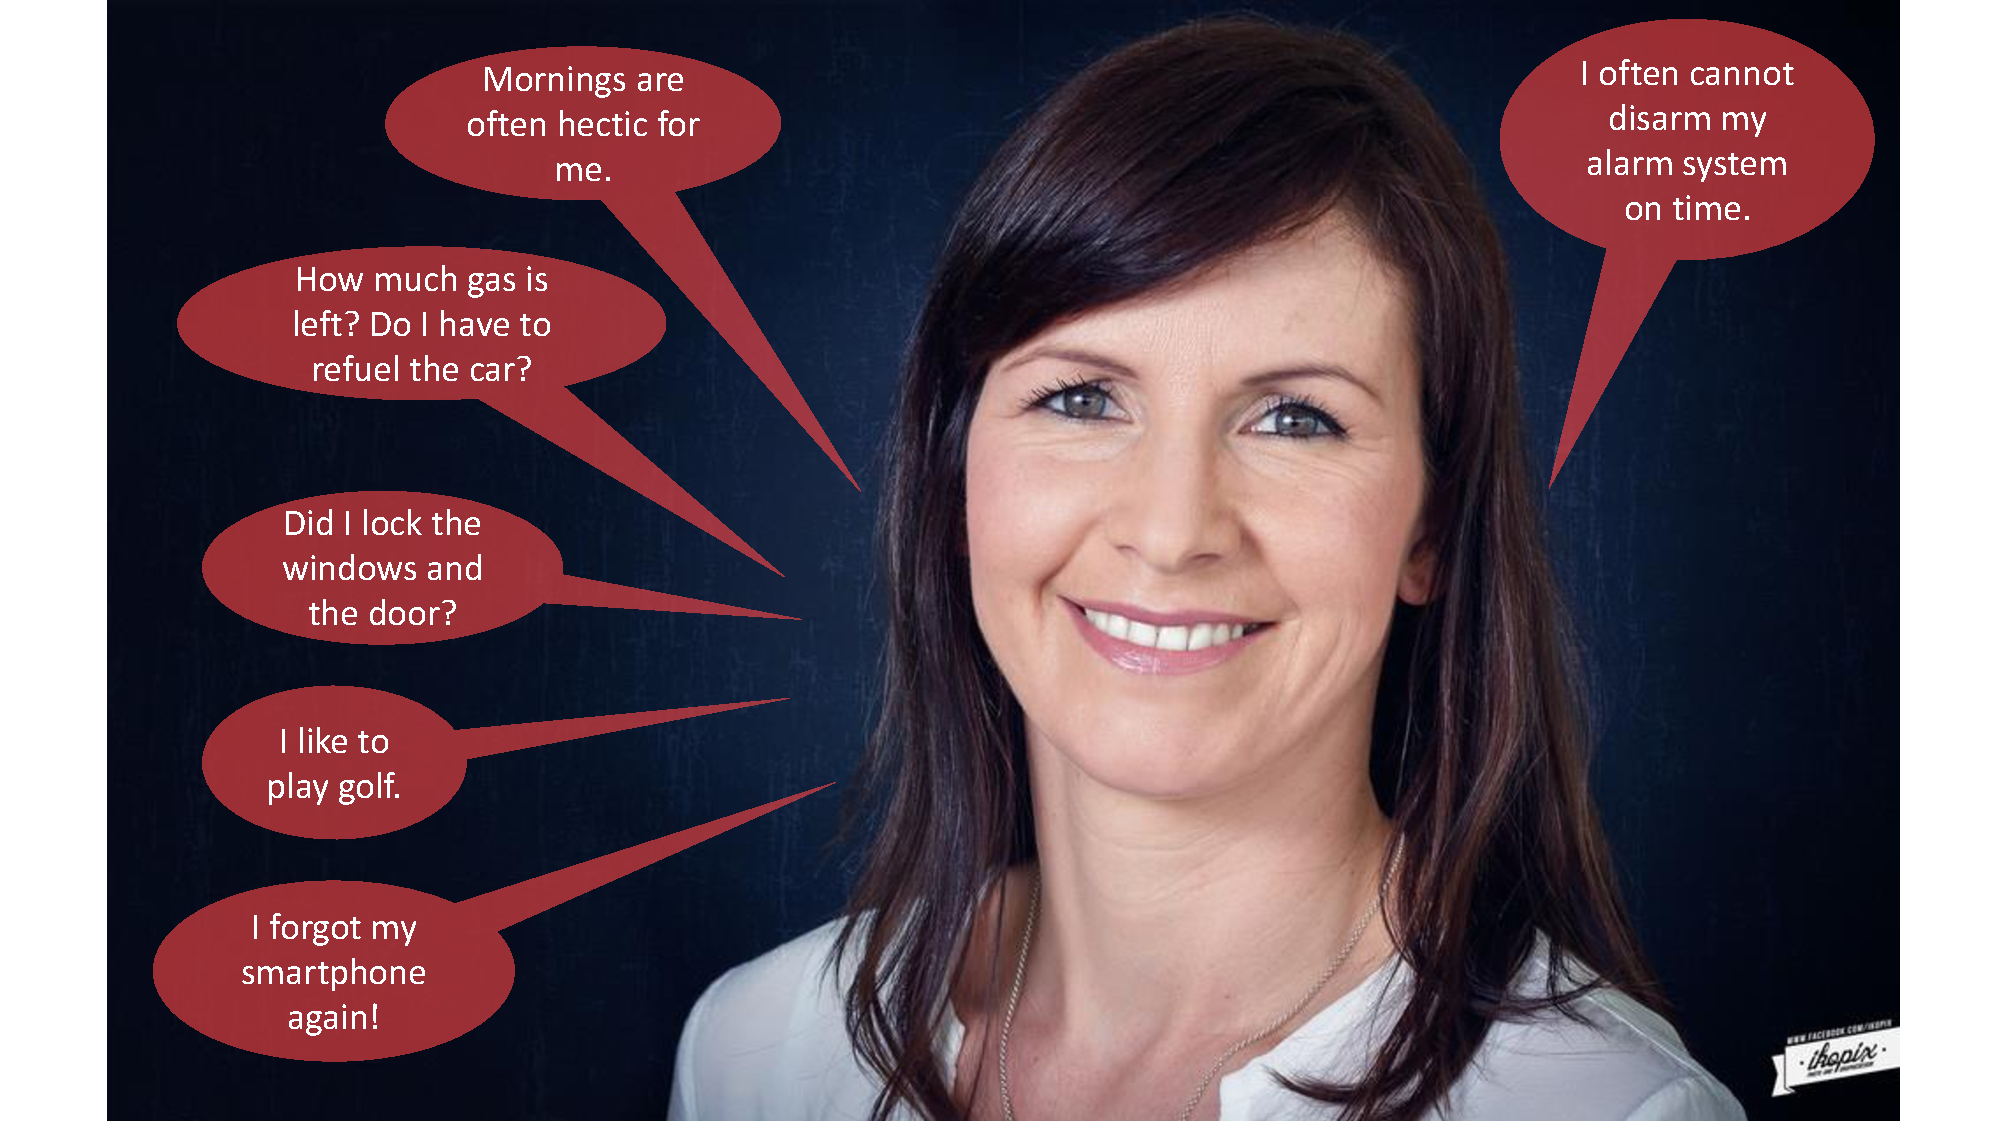
\includegraphics[keepaspectratio, width=5.5in]{Figures/Needfinding/Persona_Linda}
	\caption{Persona Linda Becker\protect\footnotemark}
	\label{fig:persona}
\end{figure}

\footnotetext{Taken from \url{http://www.flickr.com/photos/96071098@N06/17244109369} on March 15th 2016 (license: \url{https://creativecommons.org/licenses/by-nc-sa/2.0/)}}

Disarming the system is similarly painful since it requires Linda to input a code into a panel next to the door. She has to do so within 30 seconds, otherwise the alarm will go off. This happens more frequently to her because she often has her hands packed full with her purse, her daughter's school bag and newly bought groceries when she comes home. This is very annoying and a big pain point for her since it causes extra work and keeps her from really arriving at home and having some time to catch a breath after a long day at work.

Because both Linda and her husband have jobs with high responsibilities and her daughter has to go to school, the mornings with them are often hectic. Many things need to be done and organized such as preparing breakfast, doing housework, packing bags and planning the day for the family. This causes Linda to have to remember a lot of things each day and in consequence she frequently forgets to take everything with her that she needs when she leaves the house. She frequently forgets her smart phone or the charger for her laptop and only notices it when she is already in the car or even at work which can be very frustrating and costs her a lot of time. Also, she likes to play golf now and then for which she always has to pack her sports bag. This sports bag contains many items she needs among which are multiple things she has in her normal workday bag too so she has to repack the bags whenever she goes to sports. In consequence and in combination with her full and hectic days, she does not always remember to pack everything which again is frustrating and time-consuming in the end.